% Provenance (never printed): cycle 3 / 6e "La planete Terre" (rocks and
% minerals; the three rock families; recognising common rocks); see
% sources/book1/PROVENANCE.md. Book 1, grade 6, chapter 3.
% Vocabulary guard: "magma" not before g7.2 (here "molten rock");
% "sediment" not before g7.4 (here "grains of sand and mud").
\chapter{Gesteenten en mineralen}\label{ch:g6:rocks-and-minerals}

Sam buigt zich met een loep over het aanrecht. De gepolijste steen, die van
ver grijs lijkt, verandert in een menigte spikkels: roze, witte, glazig
grijze en piepkleine zwarte die glanzen als het licht erop valt. Elke
spikkel heeft vlakke, glimmende zijvlakken, en de spikkels passen in
elkaar als de stukjes van een legpuzzel. Wat zijn het?

\begin{omfigure}
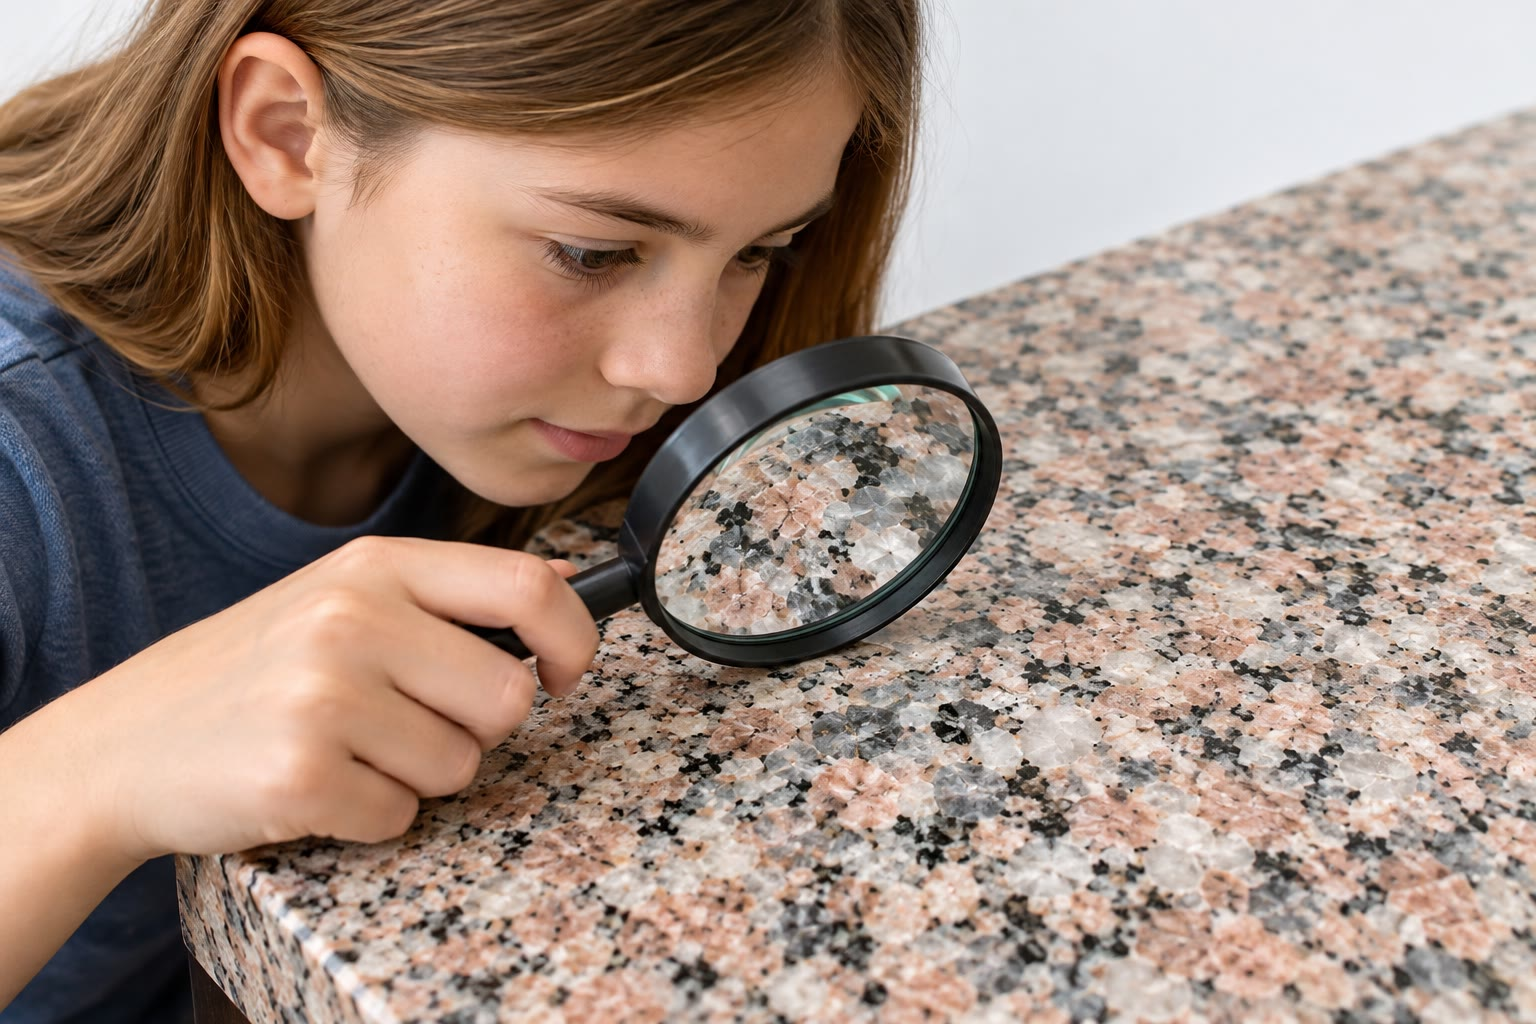
\includegraphics[width=0.6\linewidth]{images/book1/ai/g6-hand-lens-worktop.jpg}

{\small Een gespikkeld stenen aanrecht bekijken door een loep.
(AI-illustratie.)}
\end{omfigure}

\begin{recall}
\omterm{def:g3:stones-pebbles-sand:rock}{Gesteenten} zijn het harde materiaal van de aardkorst: ze kunnen in stenen
worden gebroken, door \omterm{def:g1:landscapes-around-us:water}{rivieren} tot \omterm{def:g3:stones-pebbles-sand:pebble}{kiezels} worden gerold en tot \omterm{def:g3:stones-pebbles-sand:sand}{zand} worden
vermalen (\cref{ch:g3:stones-pebbles-sand}). Water, ijs en wind slijten
\omterm{def:g3:stones-pebbles-sand:rock}{gesteenten} af (\omterm{def:g5:water-shapes-the-land:weathering}{verwering}), voeren de stukken weg (\omterm{def:g5:water-shapes-the-land:erosion}{erosie}) en laten ze
verderop vallen (\omterm{def:g5:water-shapes-the-land:deposition}{afzetting}) (\cref{ch:g5:water-shapes-the-land}). Bij een
\omterm{def:g4:volcanoes-earthquakes-first-look:volcano}{vulkaan} komt gesmolten \omterm{def:g3:stones-pebbles-sand:rock}{gesteente} naar buiten als \omterm{def:g4:volcanoes-earthquakes-first-look:eruption}{lava}
(\cref{ch:g4:volcanoes-earthquakes-first-look}).
\end{recall}

\section{Een gesteente bestaat uit mineralen}

De spikkels van het aanrecht zijn \omterm{def:g6:rocks-and-minerals:mineral}{mineralen}, en de steen is een graniet.

\begin{definition}[Mineraal]\label{def:g6:rocks-and-minerals:mineral}
Een \emph{mineraal}\index{mineraal} is een natuurlijke vaste stof, niet
gemaakt door levende wezens, altijd met dezelfde samenstelling en met
atomen die op een regelmatige manier geordend zijn. Een \emph{\omterm{def:g3:stones-pebbles-sand:rock}{gesteente}}
bestaat uit één mineraal of, vaker, uit verschillende mineralen die aan
elkaar vastzitten.
% ledger: usgs:mineral-rock
\end{definition}

Graniet bestaat vooral uit drie \omterm{def:g6:rocks-and-minerals:mineral}{mineralen}: \emph{veldspaat} (roze of wit),
\emph{kwarts} (grijs en glazig) en \emph{mica} (zwart of zilverachtig, in
dunne glimmende schilfers). Andere \omterm{def:g3:stones-pebbles-sand:rock}{gesteenten} bestaan uit één enkel
\omterm{def:g6:rocks-and-minerals:mineral}{mineraal}: kalksteen bijvoorbeeld bestaat bijna alleen uit calciet.
% ledger: nps:granite-minerals, usgs:mineral-rock

\begin{omfigure}
\begin{minipage}[c]{0.5\linewidth}\centering
\begin{tikzpicture}
  \begin{axis}[axis equal image, hide axis, width=\linewidth,
      xmin=0, xmax=6, ymin=0, ymax=4]
    \addplot[fill=orange!35!pink, draw=black!55, line width=0.4pt]
      table {figdata/out/grade-6-granite_mosaic-feldspar.dat};
    \addplot[fill=black!12, draw=black!55, line width=0.4pt]
      table {figdata/out/grade-6-granite_mosaic-quartz.dat};
    \addplot[fill=black!85, draw=black!55, line width=0.4pt]
      table {figdata/out/grade-6-granite_mosaic-mica.dat};
  \end{axis}
\end{tikzpicture}

{\small \tikz\fill[orange!35!pink, draw=black!55] (0,0) rectangle (0.25,0.18); veldspaat\quad
\tikz\fill[black!12, draw=black!55] (0,0) rectangle (0.25,0.18); kwarts\quad
\tikz\fill[black!85] (0,0) rectangle (0.25,0.18); mica}
\end{minipage}\hfill
\begin{minipage}[c]{0.46\linewidth}\centering
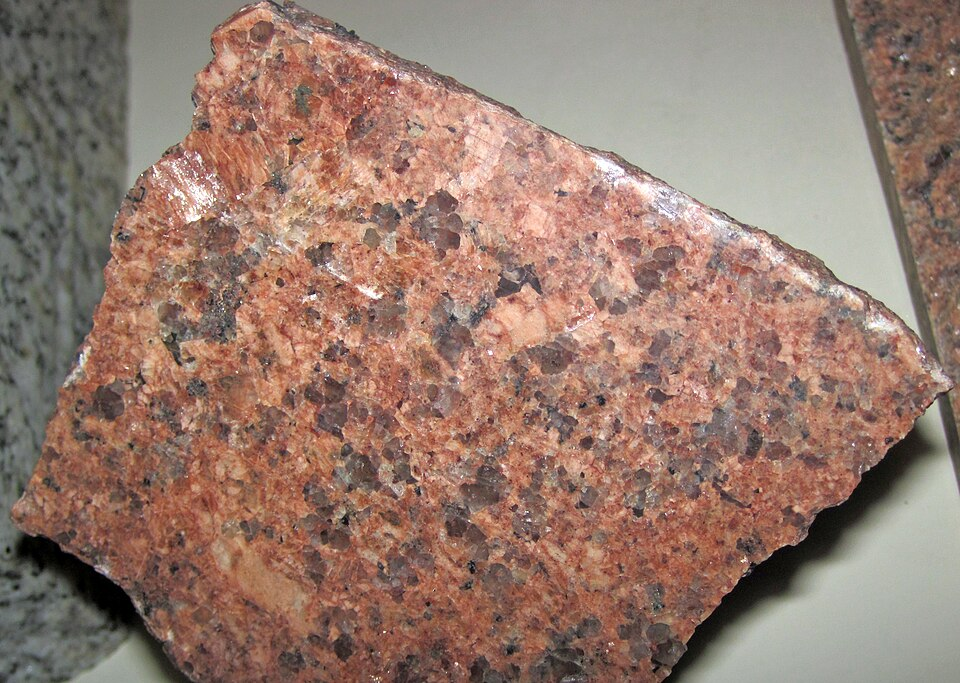
\includegraphics[width=\linewidth]{images/book1/g6-granite.jpg}
\end{minipage}

\smallskip
{\small Links: graniet getekend als een mozaïek van korrels, elke korrel
één \omterm{def:g6:rocks-and-minerals:mineral}{mineraal} (een vergroting, niet op schaal). Rechts: een echt roze
graniet, ongeveer zo groot als een hand. (Foto: James St.~John, CC BY 2.0,
via Wikimedia Commons.)}
% ledger: nps:granite-minerals, commons:jsj-rocks (figdata/grade-6/granite_mosaic.py)
\end{omfigure}

\section{Kristallen}

Onder de loep laten veel mineraalkorrels vlakke, glimmende zijvlakken en
rechte randen zien. Waar een \omterm{def:g6:rocks-and-minerals:mineral}{mineraal} de ruimte heeft gehad om vrij te
groeien, in een holte van het \omterm{def:g3:stones-pebbles-sand:rock}{gesteente}, vormt het een kristal: een vaste
stof met een regelmatige vorm, begrensd door vlakke zijvlakken. Die vorm
komt van de regelmatige ordening van zijn atomen, die in de scheikundeboeken
wordt bestudeerd. Een kwartskristal bijvoorbeeld is een zuil met zes
zijden die in een punt eindigt; een micakristal splijt in velletjes die
dunner zijn dan papier.

\begin{omfigure}
\begin{minipage}[c]{0.2\linewidth}\centering
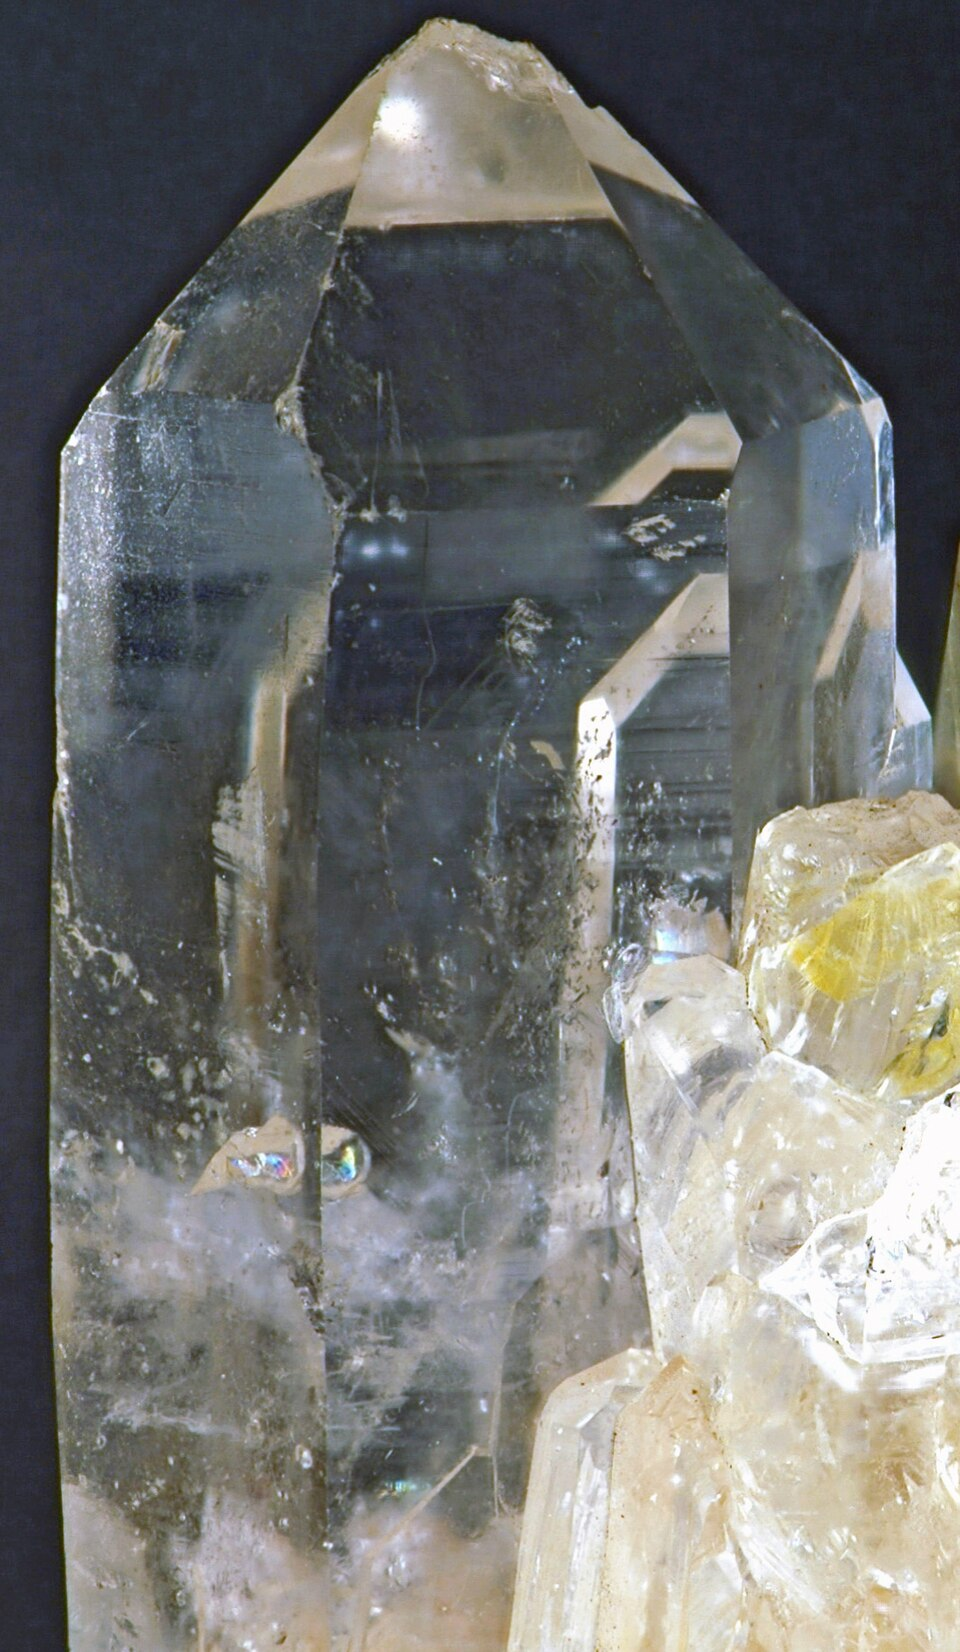
\includegraphics[height=4.2cm]{images/book1/g6-quartz.jpg}
\end{minipage}\hfill
\begin{minipage}[c]{0.44\linewidth}\centering
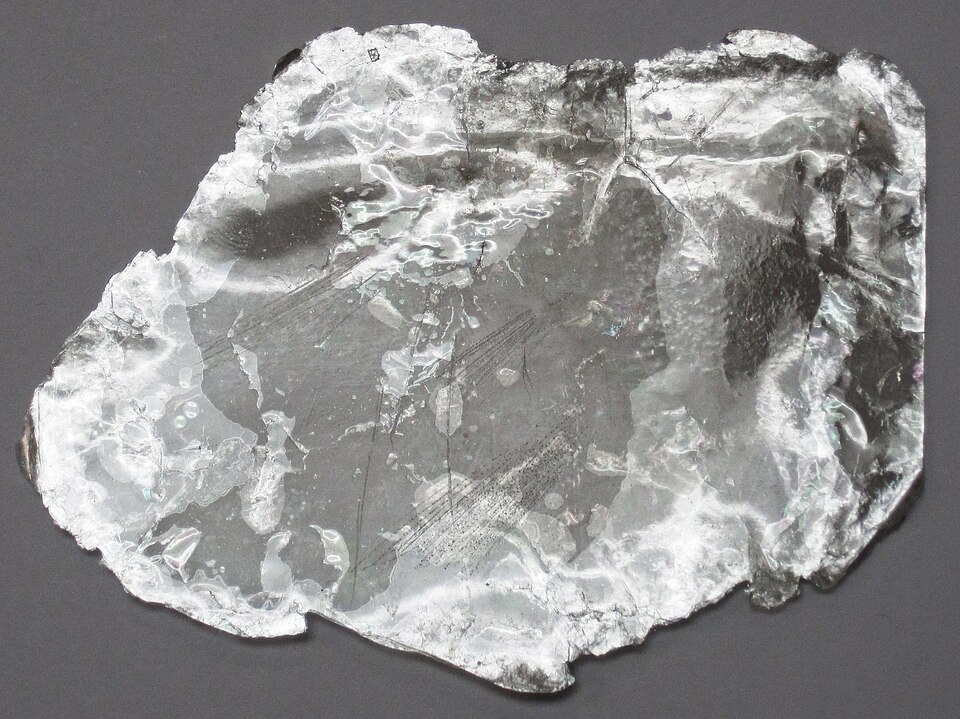
\includegraphics[height=4.2cm]{images/book1/g6-mica.jpg}
\end{minipage}\hfill
\begin{minipage}[c]{0.28\linewidth}
{\small Links: een kwartskristal, met zijn vlakke zijvlakken. Rechts: een
velletje mica, een \omterm{def:g6:rocks-and-minerals:mineral}{mineraal} dat in heel dunne schilfers splijt. (Foto's:
James St.~John, CC BY 2.0, via Wikimedia Commons.)}
% ledger: commons:jsj-rocks
\end{minipage}
\end{omfigure}

In graniet groeiden de korrels tegen elkaar aan gedrukt, dus hebben ze geen
mooie vorm: ze passen in elkaar als een legpuzzel. Hun grootte vertelt een
verhaal. Graniet ontstaat diep onder de grond, waar gesmolten \omterm{def:g3:stones-pebbles-sand:rock}{gesteente}
heel langzaam afkoelt: de korrels krijgen de tijd om groot genoeg te
groeien om ze met het blote oog te zien. Gesmolten \omterm{def:g3:stones-pebbles-sand:rock}{gesteente} dat snel
afkoelt aan het oppervlak, als \omterm{def:g4:volcanoes-earthquakes-first-look:eruption}{lava}, geeft \omterm{def:g3:stones-pebbles-sand:rock}{gesteenten} met korrels die te
klein zijn om te zien.
% ledger: usgs:mineral-rock

\section{De drie families van gesteenten}

Geologen delen \omterm{def:g3:stones-pebbles-sand:rock}{gesteenten} in drie families in, niet naar hun kleur, maar
naar de manier waarop ze zijn ontstaan.

\begin{definition}[De drie families van gesteenten]\label{def:g6:rocks-and-minerals:rock-families}
Een \emph{stollingsgesteente}\index{stollingsgesteente} ontstaat als
gesmolten \omterm{def:g3:stones-pebbles-sand:rock}{gesteente} afkoelt en vast wordt: graniet diep onder de grond,
basalt uit \omterm{def:g4:volcanoes-earthquakes-first-look:eruption}{lava}. Een \emph{afzettingsgesteente}\index{afzettingsgesteente}
ontstaat aan het aardoppervlak uit korrels \omterm{def:g3:stones-pebbles-sand:sand}{zand} en \omterm{def:g3:stones-pebbles-sand:sand}{slib}, of uit de
schelpen van levende wezens, die in lagen zijn neergelegd en daarna hard
zijn geworden: zandsteen, schalie, kalksteen. Een \emph{metamorf
gesteente}\index{metamorf gesteente} is een \omterm{def:g3:stones-pebbles-sand:rock}{gesteente} dat zonder te smelten
is omgevormd door warmte en druk diep onder de grond: marmer (uit
kalksteen), leisteen (uit schalie).
% ledger: usgs:mineral-rock, usgs:sedimentary, usgs:metamorphic, geo:marble, geo:slate
\end{definition}

De naam \emph{\omterm{def:g6:rocks-and-minerals:rock-families}{stollingsgesteente}} zegt het al: het is gestold uit een
smelt. \omterm{def:g6:rocks-and-minerals:rock-families}{Afzettingsgesteenten} laten vaak lagen zien, de een boven op de
ander, zoals de bladzijden van een boek. Metamorfe \omterm{def:g3:stones-pebbles-sand:rock}{gesteenten} zijn vaak
samengeperst en geplooid; sommige, zoals leisteen, splijten in vlakke
platen.
% ledger: usgs:mineral-rock, usgs:sedimentary, usgs:metamorphic

Veel \omterm{def:g6:rocks-and-minerals:rock-families}{afzettingsgesteenten} bestaan uit de korrels die je in
\cref{ch:g3:stones-pebbles-sand} op grootte hebt gesorteerd: \omterm{def:g3:stones-pebbles-sand:pebble}{kiezels} en
\omterm{def:g3:stones-pebbles-sand:pebble}{grind}, \omterm{def:g3:stones-pebbles-sand:sand}{zand}, \omterm{def:g3:stones-pebbles-sand:sand}{slib}. Als ze eenmaal begraven zijn, verliezen de korrels hun
water en worden ze aan elkaar gekit door een natuurlijk cement. De grootte
van de korrels geeft het \omterm{def:g3:stones-pebbles-sand:rock}{gesteente} zijn naam.
% ledger: usgs:sedimentary, usgs:wentworth

\begin{omfigure}
\begin{tikzpicture}[
    col/.style={draw=black!60, rounded corners=2pt, minimum width=3.6cm, minimum height=1.9cm},
    lab/.style={font=\scriptsize, align=center}]
  % gravel -> conglomerate
  \node[col, fill=omLithCongl!50] (g) at (0,0) {};
  \foreach \x/\y/\r in {-1.2/0.4/0.32, -0.4/-0.3/0.4, 0.5/0.35/0.3, 1.25/-0.35/0.33, 0.2/-0.55/0.18, -1.3/-0.5/0.22}
    \fill[gray!55, draw=black!60] (\x,\y) circle (\r);
  \node[lab, above=2pt] at (g.north) {\textbf{grind}\\ meer dan 2~mm};
  \node[lab, below=3pt] (cg) at (g.south) {$\downarrow$ begraven en gekit\\ \textbf{conglomeraat}};
    % sand -> sandstone
  \pgfmathsetseed{7}

  \node[col, fill=omLithSand!60] (s) at (4.2,0) {};
  \foreach \i in {1,...,70} \fill[brown!60!black] ({4.2+1.65*rand},{0.82*rand}) circle (0.045);
  \node[lab, above=2pt] at (s.north) {\textbf{zand}\\ 2~mm tot $\frac{1}{16}$~mm};
  \node[lab, below=3pt] at (s.south) {$\downarrow$ begraven en gekit\\ \textbf{zandsteen}};
  % mud -> shale
  \node[col, fill=omLithShale!70] (m) at (8.4,0) {};
  \foreach \y in {-0.75,-0.5,...,0.8} \draw[black!35, line width=0.3pt] (6.75,\y) -- (10.05,\y);
  \node[lab, above=2pt] at (m.north) {\textbf{slib} (silt en klei)\\ minder dan $\frac{1}{16}$~mm};
  \node[lab, below=3pt] at (m.south) {$\downarrow$ begraven en samengeperst\\ \textbf{schalie}};
\end{tikzpicture}

{\small Drie \omterm{def:g6:rocks-and-minerals:rock-families}{afzettingsgesteenten}, genoemd naar de grootte van hun korrels
(korrels sterk vergroot; het \omterm{def:g3:stones-pebbles-sand:sand}{zand} getekend op de schaal van het vak, het
\omterm{def:g3:stones-pebbles-sand:pebble}{grind} groter).}
% ledger: usgs:wentworth, usgs:sedimentary
\end{omfigure}

\begin{inthefield}[De stenen van een stad lezen]
Steden zijn verzamelingen \omterm{def:g3:stones-pebbles-sand:rock}{gesteenten} in de open lucht. Loop met een
volwassene langs oude muren, trappen, beelden, kerkgevels en bestrating, en
kijk goed, zonder iets te krassen of te breken. Sommige stoepranden en
traptreden zijn van graniet: zoek het glazige kwarts en de glimmende mica.
Veel oude muren en gevels zijn van kalksteen of zandsteen: zoek naar
schelpen, of wrijf met een vingertop over een afgevallen kruimel zandsteen
om het \omterm{def:g3:stones-pebbles-sand:sand}{zand} te voelen. Daken kunnen van leisteen zijn, gespleten in dunne
platen. Noteer in een schrift waar elke steen zit, welke kleur hij heeft,
hoe zijn korrels eruitzien en tot welke familie hij volgens jou hoort; een
foto helpt om later te vergelijken met de tabel van dit hoofdstuk.
\end{inthefield}

\section{De kringloop van gesteenten}

\omterm{def:g3:stones-pebbles-sand:rock}{Gesteenten} zijn niet eeuwig. Een granieten \omterm{def:g1:landscapes-around-us:landform}{berg} verweert langzaam; zijn
korrels worden door \omterm{def:g1:landscapes-around-us:water}{rivieren} naar de \omterm{def:g2:water-on-earth:ocean}{zee} gevoerd en daar in lagen
neergelegd; steeds dieper begraven worden de lagen hard en veranderen ze
in zandsteen. Als het zandsteen nog dieper terechtkomt, vormen warmte en
druk het om tot een \omterm{def:g6:rocks-and-minerals:rock-families}{metamorf gesteente}; nog dieper kan het smelten, en het
gesmolten \omterm{def:g3:stones-pebbles-sand:rock}{gesteente} vormt bij het afkoelen een nieuw \omterm{def:g6:rocks-and-minerals:rock-families}{stollingsgesteente}.
Beetje bij beetje, in miljoenen jaren, gaat het materiaal van de
\omterm{def:g3:stones-pebbles-sand:rock}{gesteenten} steeds weer rond.
% ledger: usgs:sedimentary, usgs:metamorphic

\begin{definition}[Kringloop van gesteenten]\label{def:g6:rocks-and-minerals:rock-cycle}
De \emph{kringloop van gesteenten}\index{kringloop van gesteenten} is de
eindeloze reis waarbij \omterm{def:g3:stones-pebbles-sand:rock}{gesteenten} van elke familie langzaam veranderen in
\omterm{def:g3:stones-pebbles-sand:rock}{gesteenten} van de andere families: door \omterm{def:g5:water-shapes-the-land:weathering}{verwering} en \omterm{def:g5:water-shapes-the-land:erosion}{erosie} aan het
oppervlak, door begraving en verharding, door warmte en druk, door smelten
en afkoelen.
\end{definition}

\begin{omfigure}
\begin{tikzpicture}[
    fam/.style={draw, rounded corners=4pt, thick, align=center, minimum width=3.2cm,
                minimum height=1.0cm, font=\small\bfseries},
    stage/.style={draw, dashed, rounded corners=4pt, align=center, minimum width=3.0cm,
                  minimum height=0.9cm, font=\small},
    arr/.style={-{Stealth[length=2.6mm]}, thick},
    lab/.style={font=\scriptsize, align=center, fill=white, inner sep=1.5pt}]
  \node[fam, fill=omLithGranite!60] (ign) at (0,3.6) {stollingsgesteenten\\[-1pt]{\normalfont\scriptsize graniet, basalt}};
  \node[stage, fill=orange!15] (grains) at (6.6,3.6) {korrels zand\\en slib};
  \node[fam, fill=omLithSand!70] (sed) at (6.6,0) {afzettingsgesteenten\\[-1pt]{\normalfont\scriptsize zandsteen, schalie, kalksteen}};
  \node[fam, fill=omLithSchist!60] (met) at (0,0) {metamorfe gesteenten\\[-1pt]{\normalfont\scriptsize marmer, leisteen}};
  \node[stage, fill=red!12] (melt) at (-4.2,1.8) {gesmolten gesteente\\diep onder de grond};
  \draw[arr] (ign) -- node[lab, above] {verwering\\en erosie} (grains);
  \draw[arr] (grains) -- node[lab, right] {in lagen neergelegd,\\begraven, verhard} (sed);
  \draw[arr] (sed) -- node[lab, below=2pt] {warmte en druk,\\diep onder de grond} (met);
  \draw[arr] (met) -- node[lab, below left] {smelten} (melt);
  \draw[arr] (melt) -- node[lab, above left] {afkoelen} (ign);
  \draw[arr, black!55] (met.north east) to[bend left=12] node[lab, pos=0.45, left=4pt, text=black!60] {verwering} ([xshift=-6pt]grains.south west);
  \draw[arr, black!55] (sed.north west) to[bend left=10] (grains.south west);
\end{tikzpicture}

{\small De \omterm{def:g6:rocks-and-minerals:rock-cycle}{kringloop van gesteenten}. Elke pijl duurt duizenden tot
miljoenen jaren. Elk \omterm{def:g3:stones-pebbles-sand:rock}{gesteente} dat aan het oppervlak komt, kan verweren
(grijze pijlen).}
% ledger: usgs:sedimentary, usgs:metamorphic, usgs:mineral-rock
\end{omfigure}

\section{Gewone gesteenten herkennen}

Hier zijn zeven \omterm{def:g3:stones-pebbles-sand:rock}{gesteenten} die je vaak tegenkomt in gebouwen, bestrating
en \omterm{def:g1:landscapes-around-us:landscape}{landschappen}.

\begin{omfigure}
\newcommand{\gsixrock}[2]{\begin{minipage}[t]{0.235\linewidth}\centering
  \includegraphics[width=\linewidth, height=0.72\linewidth, keepaspectratio=false]{images/book1/#1}\\[1pt]
  {\footnotesize #2}\end{minipage}}
\gsixrock{g6-granite.jpg}{graniet}\hfill
\gsixrock{g6-basalt.jpg}{basalt}\hfill
\gsixrock{g6-sandstone.jpg}{zandsteen}\hfill
\gsixrock{g6-limestone.jpg}{kalksteen (met schelpen)}\par\medskip
\gsixrock{g6-shale.jpg}{schalie}\hspace{0.02\linewidth}%
\gsixrock{g6-marble.jpg}{marmer}\hspace{0.02\linewidth}%
\gsixrock{g6-slate-roof.jpg}{leisteen, op een dak}

\medskip
{\small Zeven gewone \omterm{def:g3:stones-pebbles-sand:rock}{gesteenten}. (Foto's: James St.~John, CC BY 2.0; dak:
Øyvind Holmstad, CC0; via Wikimedia Commons.)}
% ledger: commons:jsj-rocks, commons:roof-slates
\end{omfigure}

\begin{center}
\small
\begin{tabular}{>{\raggedright\arraybackslash}p{0.13\linewidth}>{\raggedright\arraybackslash}p{0.15\linewidth}>{\raggedright\arraybackslash}p{0.6\linewidth}}
\hline
\omterm{def:g3:stones-pebbles-sand:rock}{gesteente} & familie & waar je op let\\
\hline
graniet & stolling & grote korrels van verschillende kleuren: roze of witte veldspaat, grijs glazig kwarts, zwarte glimmende mica\\
basalt & stolling & donkergrijs tot zwart, korrels te klein om te zien, vaak kleine ronde gaatjes van gasbelletjes\\
zandsteen & \omterm{def:g5:water-shapes-the-land:deposition}{afzetting} & zandkorrels die je kunt voelen, ruw als schuurpapier\\
kalksteen & \omterm{def:g5:water-shapes-the-land:deposition}{afzetting} & licht van kleur, vaak met schelpen; bruist onder een druppel verdund zuur\\
schalie & \omterm{def:g5:water-shapes-the-land:deposition}{afzetting} & heel fijn en zacht, gemaakt van verhard \omterm{def:g3:stones-pebbles-sand:sand}{slib} (klei); in dunne laagjes\\
marmer & metamorf & wit of gekleurd, gemaakt van glimmende kristallen die schitteren als suiker; bruist onder zuur\\
leisteen & metamorf & grijs, heel fijn, splijt in dunne, harde, vlakke platen\\
\hline
\end{tabular}
% ledger: nps:granite-minerals, geo:basalt, usgs:sedimentary, geo:limestone, geo:marble, geo:slate
\end{center}

\begin{safety}
De zuurtest wordt alleen door een volwassene gedaan, met een veiligheidsbril
en handschoenen, met een heel verdund zuur. Proef nooit aan een steen of
een poeder, en breek nooit stenen met gereedschap: kijken door een loep
vertelt al heel veel.
% ledger: geo:limestone
\end{safety}

Een determineertabel is een lijst vragen, elk met twee antwoorden, die je
stap voor stap naar de naam van een \omterm{def:g3:stones-pebbles-sand:rock}{gesteente} leidt.

\begin{omfigure}
\begin{tikzpicture}[
    q/.style={draw, rounded corners=3pt, fill=omRecall!10, align=center, text width=3.7cm,
              font=\scriptsize, inner sep=3pt},
    r/.style={draw, rounded corners=3pt, thick, fill=omLithSand!40, font=\scriptsize\bfseries,
              align=center, minimum width=1.7cm, inner sep=3pt},
    arr/.style={-{Stealth[length=2mm]}, thick}, yn/.style={font=\scriptsize\itshape, fill=white, inner sep=1pt}]
  \node[q] (q1) at (0,0) {Bruist het onder een druppel verdund zuur?};
  \node[q] (q2) at (-3.4,-1.6) {Zie je schelpen, of ziet het er dof en fijn uit?};
  \node[r] (lime) at (-4.8,-3.4) {kalksteen};
  \node[r, align=center] (marb) at (-2.0,-3.4) {marmer\\[-1pt]{\normalfont\tiny glimmende kristallen}};
  \node[q] (q3) at (3.2,-1.6) {Zie je korrels van verschillende kleuren, roze, grijs, zwart?};
  \node[r] (gran) at (6.9,-1.6) {graniet};
  \node[q] (q4) at (3.2,-3.2) {Donker, korrels te klein om te zien, kleine ronde gaatjes?};
  \node[r] (bas) at (6.9,-3.2) {basalt};
  \node[q] (q5) at (3.2,-4.8) {Ruw als schuurpapier, gemaakt van zandkorrels?};
  \node[r] (sand) at (6.9,-4.8) {zandsteen};
  \node[q] (q6) at (3.2,-6.4) {Hard, splijt in dunne vlakke platen?};
  \node[r] (slat) at (6.9,-6.4) {leisteen};
  \node[r] (shal) at (3.2,-7.8) {schalie};
  \draw[arr] (q1) -| node[yn, pos=0.25] {ja} (q2);
  \draw[arr] (q1) -| node[yn, pos=0.25] {nee} (q3);
  \draw[arr] (q2.south-|lime) -- node[yn, right] {ja} (lime);
  \draw[arr] (q2.south-|marb) -- node[yn, right] {nee} (marb);
  \foreach \a/\b in {q3/gran, q4/bas, q5/sand, q6/slat}{\draw[arr] (\a) -- node[yn, above] {ja} (\b);}
  \foreach \a/\b in {q3/q4, q4/q5, q5/q6, q6/shal}{\draw[arr] (\a) -- node[yn, right] {nee} (\b);}
\end{tikzpicture}

{\small Een determineertabel voor de zeven \omterm{def:g3:stones-pebbles-sand:rock}{gesteenten} van de tabel. Begin
bovenaan en beantwoord elke vraag met ja of nee.}
% ledger: geo:limestone, geo:marble, nps:granite-minerals, geo:basalt, usgs:sedimentary, geo:slate
\end{omfigure}

\paragraph{Hardheid.} Nog één aanwijzing helpt om een \omterm{def:g6:rocks-and-minerals:mineral}{mineraal} te
herkennen: hoe makkelijk het te krassen is.

\begin{definition}[Hardheid en de schaal van Mohs]\label{def:g6:rocks-and-minerals:hardness}
De \emph{hardheid}\index{hardheid} van een \omterm{def:g6:rocks-and-minerals:mineral}{mineraal} is hoe goed het
weerstand biedt tegen krassen: een \omterm{def:g6:rocks-and-minerals:mineral}{mineraal} krast elk zachter \omterm{def:g6:rocks-and-minerals:mineral}{mineraal} en
wordt gekrast door elk harder \omterm{def:g6:rocks-and-minerals:mineral}{mineraal}. De \emph{schaal van
Mohs}\index{schaal van Mohs} rangschikt de hardheid van 1 tot 10 met tien
referentiemineralen, van talk (1), het zachtste, tot diamant (10), het
hardste.
% ledger: nps:mohs-ladder, nps:mohs-testers
\end{definition}

\begin{omfigure}
\begin{tikzpicture}[x=1cm, y=0.62cm]
  \draw[thick, black!60] (0,0.5) -- (0,10.5);
  \foreach \n/\m in {1/talk, 2/gips, 3/calciet, 4/fluoriet, 5/apatiet,
                     6/veldspaat (orthoklaas), 7/kwarts, 8/topaas, 9/korund, 10/diamant}{
    \fill[omRecall!25, draw=black!50] (-0.32,\n-0.32) rectangle (0.32,\n+0.32);
    \node[font=\scriptsize\bfseries] at (0,\n) {\n};
    \node[font=\scriptsize, anchor=east] at (-0.5,\n) {\m};}
  \foreach \v/\t in {2.5/vingernagel, 3.5/koperen munt, 5.5/glas, 6.5/spijker}{
    \draw[red!70!black, thick] (0.4,\v) -- (1.0,\v);
    \node[font=\scriptsize, red!70!black, anchor=west] at (1.05,\v) {\t\ (ongeveer \v)};}
  \node[font=\scriptsize\itshape, anchor=south] at (0,10.6) {harder};
  \node[font=\scriptsize\itshape, anchor=north] at (0,0.4) {zachter};
  \node[font=\scriptsize, align=left, anchor=west, text width=6.2cm] at (4.3,5.5)
    {Een vingernagel krast talk en gips, maar geen calciet. Een koperen munt
     krast calciet. Kwarts krast glas en staal; geen van de vier
     testvoorwerpen krast kwarts. Mica, met 2 tot 3, kan net met een
     vingernagel gekrast worden.};
\end{tikzpicture}

{\small De schaal van Mohs (links: de tien referentiemineralen) en vier
alledaagse testvoorwerpen (rechts, in rood).}
% ledger: nps:mohs-ladder, nps:mohs-testers, geo:mica-hardness
\end{omfigure}

\begin{method}[De krastest]\label{met:g6:rocks-and-minerals:scratch}
\begin{enumerate}
  \item Probeer het \omterm{def:g6:rocks-and-minerals:mineral}{mineraal} te krassen met je vingernagel, daarna met een
        koperen munt. (Glas en staal worden alleen door een volwassene
        gebruikt.)
  \item Wrijf met een vinger over het spoor: een echte kras blijft, een
        spoortje poeder van het testvoorwerp veeg je weg.
  \item De \omterm{def:g6:rocks-and-minerals:hardness}{hardheid} ligt tussen die van het hardste testvoorwerp dat het
        niet krast en die van het zachtste testvoorwerp dat het wel krast.
\end{enumerate}
\end{method}

\begin{example}[Kwarts of calciet?]\label{ex:g6:rocks-and-minerals:quartz-calcite}
Twee witte \omterm{def:g6:rocks-and-minerals:mineral}{mineralen} lijken op elkaar. Het eerste wordt gekrast door een
koperen munt: de \omterm{def:g6:rocks-and-minerals:hardness}{hardheid} is kleiner dan 3.5; het is calciet (3). Het
tweede wordt niet gekrast door een stalen spijker en krast glas: de
\omterm{def:g6:rocks-and-minerals:hardness}{hardheid} is groter dan 6.5; van de referentiemineralen is het kwarts (7).
% ledger: nps:mohs-ladder, nps:mohs-testers
\end{example}

\section{Oefeningen}

\begin{exercise}[$\star$]\label{exo:g6:rocks-and-minerals:1}
Tot welke familie hoort elk \omterm{def:g3:stones-pebbles-sand:rock}{gesteente}: graniet, zandsteen, marmer, basalt,
kalksteen, leisteen?
\end{exercise}

\begin{exercise}[$\star$]\label{exo:g6:rocks-and-minerals:2}
Is kwarts een \omterm{def:g6:rocks-and-minerals:mineral}{mineraal} of een \omterm{def:g3:stones-pebbles-sand:rock}{gesteente}? En graniet? Leg het verschil uit
in één zin.
\end{exercise}

\begin{exercise}[$\star$]\label{exo:g6:rocks-and-minerals:3}
Zet deze \omterm{def:g6:rocks-and-minerals:mineral}{mineralen} op volgorde, van het zachtste tot het hardste: kwarts,
talk, diamant, calciet. Welk ervan kan alle andere krassen?
\end{exercise}

\begin{exercise}[$\star$]\label{exo:g6:rocks-and-minerals:4}
Neem over en vul aan met de woorden \emph{afkoelen}, \emph{warmte en druk},
\emph{\omterm{def:g5:water-shapes-the-land:weathering}{verwering}}: ``Gesmolten \omterm{def:g3:stones-pebbles-sand:rock}{gesteente} wordt een \omterm{def:g6:rocks-and-minerals:rock-families}{stollingsgesteente} door
\ldots{} Een kalksteen wordt een marmer door \ldots{} Een graniet valt
uiteen in zandkorrels door \ldots''
\end{exercise}

\begin{exercise}[$\star\star$]\label{exo:g6:rocks-and-minerals:5}
Gebruik de determineertabel. (a) Een \omterm{def:g3:stones-pebbles-sand:rock}{gesteente} bruist niet onder zuur; het
is donker, met korrels die te klein zijn om te zien en kleine ronde
gaatjes. (b) Een \omterm{def:g3:stones-pebbles-sand:rock}{gesteente} bruist onder zuur en bestaat uit glimmende
kristallen die schitteren als suiker. (c) Een \omterm{def:g3:stones-pebbles-sand:rock}{gesteente} bruist niet; het
is ruw als schuurpapier. Noem elk \omterm{def:g3:stones-pebbles-sand:rock}{gesteente}.
\end{exercise}

\begin{exercise}[$\star\star$]\label{exo:g6:rocks-and-minerals:6}
Een \omterm{def:g6:rocks-and-minerals:mineral}{mineraal} wordt gekrast door een koperen munt, maar niet door een
vingernagel. Tussen welke twee hardheden ligt het? Welk referentiemineraal
van de schaal van Mohs zou het kunnen zijn?
\end{exercise}

\begin{exercise}[$\star\star$]\label{exo:g6:rocks-and-minerals:7}
% exercise data: figdata/grade-6/granite_mosaic.py (33 / 21 / 6 grains)
In de tekening van graniet in dit hoofdstuk staan 60 korrels: 33 van
veldspaat, 21 van kwarts en 6 van mica. Welk percentage van de korrels is
kwarts? Veldspaat? Mica? Controleer dat de drie percentages samen
100~\% zijn.
\end{exercise}

\begin{exercise}[$\star\star$]\label{exo:g6:rocks-and-minerals:8}
Graniet en basalt zijn allebei \omterm{def:g6:rocks-and-minerals:rock-families}{stollingsgesteenten}. Waarom kunnen we de
korrels van graniet met het blote oog zien, maar die van basalt niet?
\end{exercise}

\begin{exercise}[$\star\star$]\label{exo:g6:rocks-and-minerals:9}
Marmer ontstaat uit kalksteen. (a) Tot welke familie hoort elk van beide?
(b) Wat is er met de kalksteen gebeurd om hem in marmer te veranderen?
(c) Waarom bruisen ze allebei onder zuur?
\end{exercise}

\begin{exercise}[$\star\star$]\label{exo:g6:rocks-and-minerals:10}
Gebruik de schaal van Mohs: (a) kan kwarts een glazen fles krassen? (b) Kan
fluoriet dat? (c) Kan een stalen spijker veldspaat krassen?
\end{exercise}

\begin{exercise}[$\star\star\star$]\label{exo:g6:rocks-and-minerals:11}
Vertel de reis van een kwartskorrel, in vijf stappen, van een granieten
\omterm{def:g1:landscapes-around-us:landform}{berg} tot een \omterm{def:g6:rocks-and-minerals:rock-families}{metamorf gesteente}. Noem bij elke stap het proces, en de
familie van het \omterm{def:g3:stones-pebbles-sand:rock}{gesteente} aan het begin en aan het eind.
\end{exercise}

\begin{exercise}[$\star\star\star$]\label{exo:g6:rocks-and-minerals:12}
Een grijs glazig \omterm{def:g6:rocks-and-minerals:mineral}{mineraal} wordt niet gekrast door een stalen spijker, krast
glas, en wordt gekrast door topaas. (a) Wat is de \omterm{def:g6:rocks-and-minerals:hardness}{hardheid} op de schaal
van Mohs? Noem het \omterm{def:g6:rocks-and-minerals:mineral}{mineraal}. (b) Zandkorrels worden jarenlang door golven en
\omterm{def:g1:landscapes-around-us:water}{rivieren} gerold. Leg met de \omterm{def:g6:rocks-and-minerals:hardness}{hardheid} uit waarom korrels van dit \omterm{def:g6:rocks-and-minerals:mineral}{mineraal}
veel langer meegaan dan korrels van calciet of mica.
\end{exercise}

\section{Probleem: De stenen van het stadsplein}

\begin{problem}[{Weekendprobleem --- de gesteenten van een stadsplein, het
hardste mineraal ertussen, en hoeveel families van gesteenten er zijn}]
\label{pb:g6:rocks-and-minerals:1}
% ledger: nps:granite-minerals, geo:limestone, geo:slate, geo:marble, nps:mohs-ladder, nps:mohs-testers, geo:mica-hardness
Op een schoolreisje bekijkt de klas de stenen van het oude stadsplein
(alleen kijken: niemand breekt of krast de monumenten). De leraar heeft
losse stukken van dezelfde stenen meegenomen van de werkplaats van de
steenhouwer, voor de hardheidstests.

\smallskip
\noindent\textbf{De fontein}: het bekken laat grote korrels zien, roze,
        wit, grijs en glazig, en zwart en glimmend.
\textbf{De bestrating}: lichte platen waarin je kleine fossiele
        schelpen ziet; een druppel verdund zuur, die de leraar op een los
        stuk doet, bruist.
\textbf{Het dak van het stadhuis}: dunne, vlakke, grijze platen van
        een heel fijnkorrelige steen.
\textbf{Het beeld}: een witte steen van glimmende kristallen die
        schitteren als suiker; hij bruist ook.

\medskip
\noindent\textbf{Deel I --- De fontein, de bestrating, het dak.}
\begin{enumerate}
  \item Noem het \omterm{def:g3:stones-pebbles-sand:rock}{gesteente} van de fontein en zijn familie. Noem de drie
        \omterm{def:g6:rocks-and-minerals:mineral}{mineralen} ervan.
  \item Noem het \omterm{def:g3:stones-pebbles-sand:rock}{gesteente} van de bestrating en zijn familie. Wat waren
        de schelpen voordat ze in de steen zaten?
  \item Noem het \omterm{def:g3:stones-pebbles-sand:rock}{gesteente} van het dak en zijn familie. Uit welk
        \omterm{def:g3:stones-pebbles-sand:rock}{gesteente} is het ontstaan?
  \item Noem het \omterm{def:g3:stones-pebbles-sand:rock}{gesteente} van het beeld en zijn familie. Uit welk
        \omterm{def:g3:stones-pebbles-sand:rock}{gesteente} is het ontstaan?
\end{enumerate}

\medskip
\noindent\textbf{Deel II --- Een hardheidstest.}
\begin{enumerate}[resume]
  \item De leraar probeert een grijze glazige korrel van de fontein te
        krassen met een stalen spijker: geen kras. De korrel krast glas.
        Welk \omterm{def:g6:rocks-and-minerals:mineral}{mineraal} is dit, en wat is de \omterm{def:g6:rocks-and-minerals:hardness}{hardheid}?
  \item De roze korrels worden gekrast door de stalen spijker, maar niet
        door glas. Tussen welke twee waarden ligt hun \omterm{def:g6:rocks-and-minerals:hardness}{hardheid}? Welk
        \omterm{def:g6:rocks-and-minerals:mineral}{mineraal} van de schaal van Mohs is het?
  \item De zwarte schilfers kunnen net met een vingernagel gekrast worden.
        Welk \omterm{def:g6:rocks-and-minerals:mineral}{mineraal} is het?
  \item Kan een koperen munt de bestrating krassen? Leg uit met de
        \omterm{def:g6:rocks-and-minerals:hardness}{hardheid} van calciet.
\end{enumerate}

\medskip
\noindent\textbf{Deel III --- De kringloop van gesteenten.}
\begin{enumerate}[resume]
  \item Na eeuwen \omterm{def:g4:clouds-rain-snow:precipitation}{regen} heeft het beeld zijn fijne details verloren. Welk
        proces van de \omterm{def:g6:rocks-and-minerals:rock-cycle}{kringloop van gesteenten} is aan het werk?
  \item Het graniet van de fontein kwam uit een \omterm{def:g1:landscapes-around-us:landform}{berg}. Wat zou er in
        miljoenen jaren van de kwartskorrels van die \omterm{def:g1:landscapes-around-us:landform}{berg} kunnen worden, en
        in welk \omterm{def:g3:stones-pebbles-sand:rock}{gesteente} zouden ze terecht kunnen komen?
  \item Hoeveel van de drie families van \omterm{def:g3:stones-pebbles-sand:rock}{gesteenten} zijn er op het plein?
        Noem het \omterm{def:g3:stones-pebbles-sand:rock}{gesteente} of de \omterm{def:g3:stones-pebbles-sand:rock}{gesteenten} van elke familie.
  \item Wat is de \omterm{def:g6:rocks-and-minerals:hardness}{hardheid} op de schaal van Mohs van het hardste \omterm{def:g6:rocks-and-minerals:mineral}{mineraal}
        in de stenen van het plein?
\end{enumerate}
\end{problem}
